\section{Arc Length, Surface Area, Volume}
In this section, we will look at four formulas built out of integrals.  Let's just get them all down here, and we'll play with them and explain them as we go!
\begin{enumerate}
\item {\bf Arc Length:} The \arclength{length of the graph of a function} $f(x)$ from the point $\left(a,f(a)\right)$ to the point $\left(b,f(b)\right)$ is given by $ L= \int_{x=a}^{x=b} \sqrt{1+\left( f'(x)\right)^2 } \dif x $.
	\begin{center}
        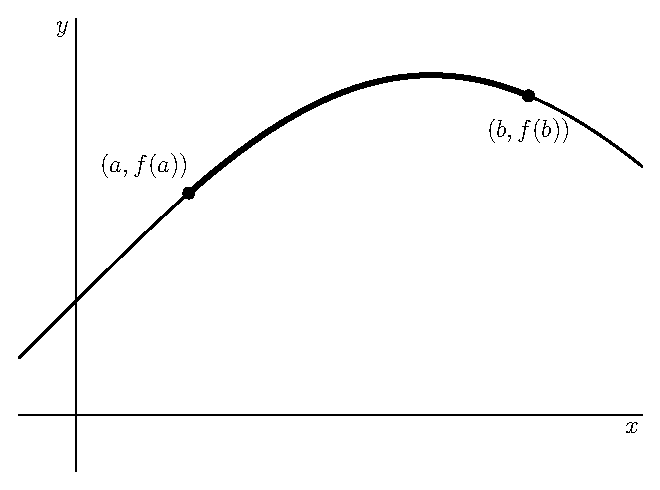
\includegraphics[width=300pt]{ChapterGeom/Figures/arclength.eps}
	\end{center}
\item {\bf Surface Area of a Surface of Revolution:} If the graph of $f(x)$ from the point $\left(a,f(a)\right)$ to the point $\left(b,f(b)\right)$ is revolved around the $y$-axis, the \area{surface area} is given by $$ SA= \int_{x=a}^{x=b} 2 \pi x\sqrt{1+\left( f'(x)\right)^2 } \dif x .$$ 
% \todo[inline]{What if it is revolved around the x axis or around another line? Or will that be covered later?}
%TODO list! :) Yes one of my todo list agenda items is to add that kind of computation in, and show how any such computation is always just a u-sub away from using the y-axis.  That a change of coordinates can always make the y-axis be your rotation axis.
	\begin{center}
        \includegraphics[width=300pt]{ChapterGeom/Figures/surfaceareaASY.eps}
	\end{center}
    
\item {\bf Volume:} We have two distinct methods for volume.

\begin{itemize}

\item {\bf Cross Sections:}  Suppose a 3D solid starts at $x=a$ and ends at $x=b$ and the function $A(x)$ represents the area of the cross-section at location $x$, then the solid has volume $V=\int_{x=a}^{x=b}A(x) \dif x $. 

	\begin{center}
		\includegraphics[width=300pt]{ChapterGeom/Figures/CrossSections.eps}
	\end{center}
\item {\bf Cylindrical Shells:}  If the region under of $f(x)$ from the point $\left(a,f(a)\right)$ to the point $\left(b,f(b)\right)$ is revolved around the $y$-axis, the volume is given by $ V= \int_{x=a}^{x=b} 2 \pi x f(x) \dif x $.
    
    \begin{center}
		\includegraphics[width=300pt]{ChapterGeom/Figures/CylindShells1.eps}
	\end{center}

\end{itemize}
\end{enumerate}

Let's now do a little example of each and throughout analyzing the example, convince ourselves that each formula is correct.

\subsection{The Arc Length Formula}\label{ArcLength}

The \integ{arc length} formula is in essence the following idea: to approximate the length of a curve, let's split it up into line segments, compute each of the line segment lengths using the Pythagorean Theorem, and then take the limit as the number of line segments goes to infinity.  Time to carry this out on a good old vanilla \conics{parabola}!
\begin{exercise}{Approximating the \arclength{Length of a Parabola} with Line Segments \Coffeecup \Coffeecup }

\begin{itemize}
\item On the axes below, graph the function $f(x)=x^2$ from the point $A=(0,0)$ to $E=(1,1)$.  Estimate the length of this arc by just connecting those two endpoints with a straight line and calculating its length via the Pythagorean Theorem.

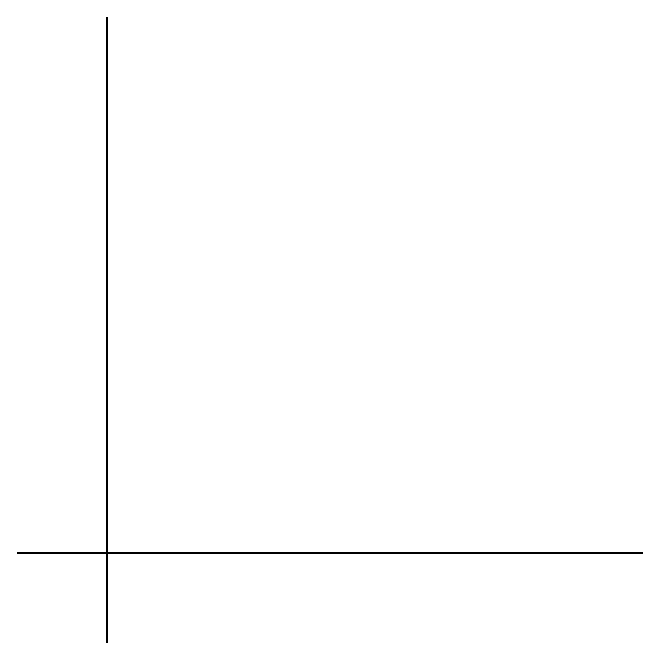
\includegraphics[scale=0.5]{quad1.eps}
\solushun{
\begin{center}
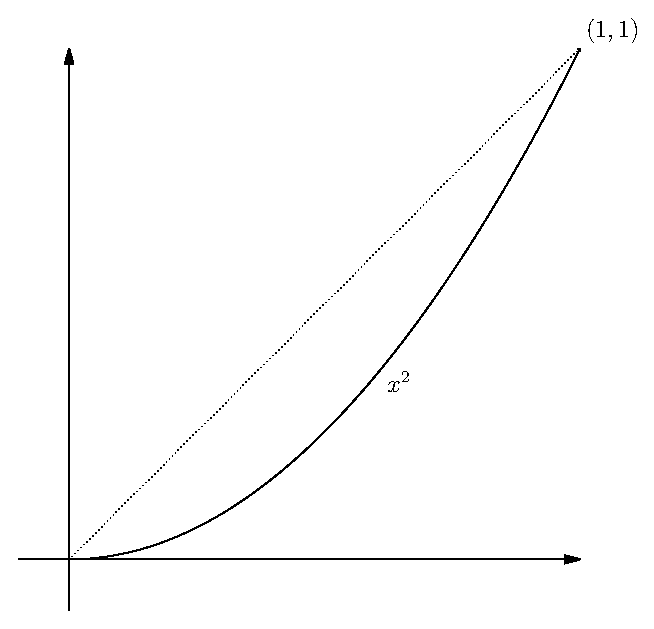
\includegraphics[scale=0.5]{ChapterGeom/Figures/squaredlength.eps}
\end{center}
The length is $\sqrt{1^2+1^2}=\sqrt{2}$.\\
}{0in}

\item Again graph the function $f(x)$ from the point $A=(0,0)$ to $E=(1,1)$, but on this graph also include a label for the point $C=(\frac{1}{2},\frac{1}{4})$.  This time lets estimate the length of this arc using two line segments.  Specifically, calculate the lengths of $\overline{AC}$ and $\overline{CE}$ and add their lengths to estimate the \parabola{arc length} of the parabola.  Did your estimate go up or down by using two segments instead of just one?  Does this make sense?

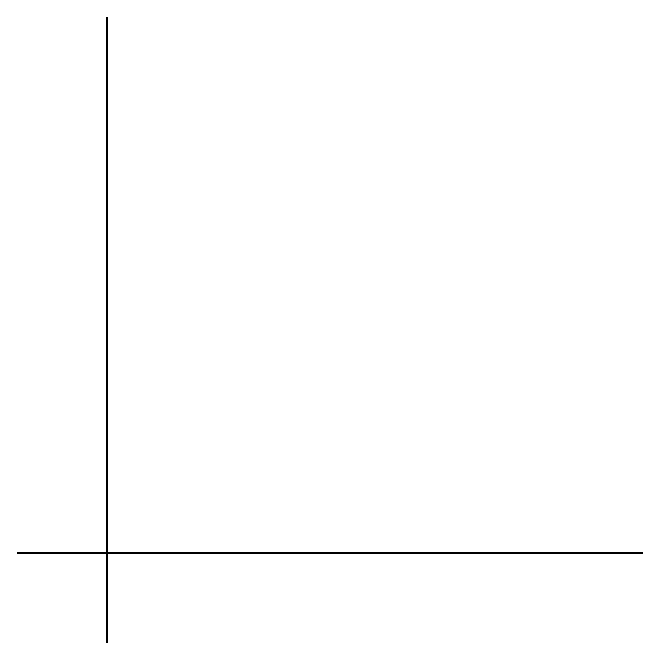
\includegraphics[scale=0.5]{quad1.eps}
\solushun{\begin{center}
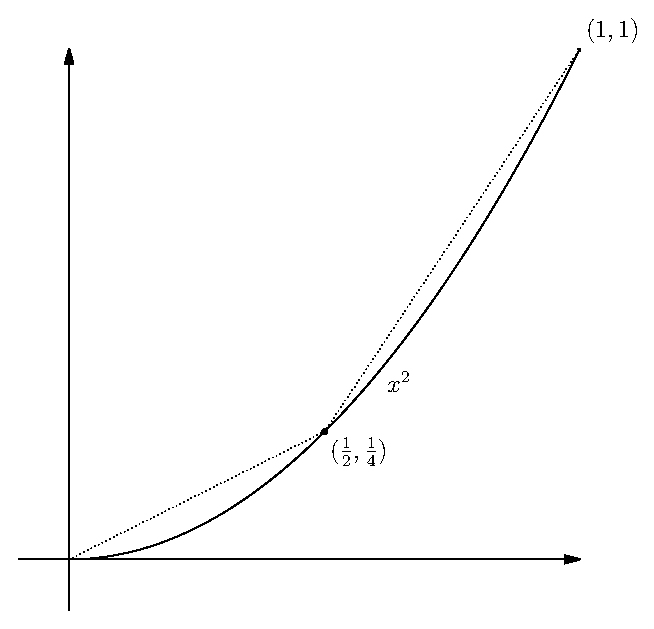
\includegraphics[scale=0.5]{ChapterGeom/Figures/squaredlength_2.eps}
\end{center}
The length is
$$
\sqrt{\left(\frac{1}{2}\right)^2+\left(\frac{1}{4}\right)^2}+\sqrt{\left(\frac{1}{2}\right)^2+\left(\frac{3}{4}\right)^2}
= \sqrt{\frac{1}{4}+\frac{1}{16}}+\sqrt{\frac{1}{4}+\frac{9}{16}}
= \sqrt{\frac{5}{16}}+\sqrt{\frac{13}{16}}
= \frac{\sqrt{5}+\sqrt{13}}{4}
$$
This is approximately $\frac{5.84}{4}\approx1.46$, which is slightly longer than $\sqrt{2}\approx1.41$. This makes sense, since the extra leg means the two paths cover more distance than the single path.\\
}{0in}

\item Define $A$, $C$, and $E$ as before.  Define $B$ to be the point on the parabola with $x$-coordinate one-fourth and $D$ to be the point on the parabola with $x$-coordinate three-fourths.  Again estimate the length of the curve by adding the lengths of the segments  $\overline{AB}$, $\overline{BC}$, $\overline{CD}$, and  $\overline{DE}$.  What happens to the estimate?  Did it increase or decrease?  Did it get more or less accurate as compared to the true arc length?

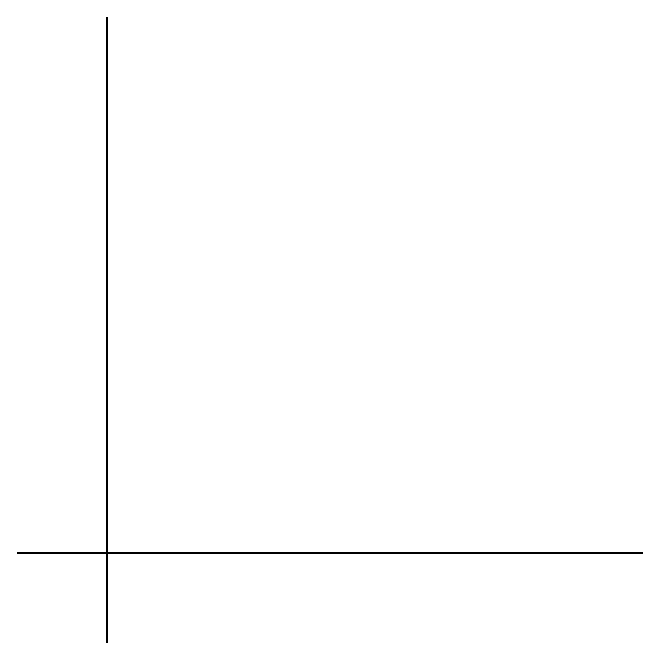
\includegraphics[scale=0.5]{quad1.eps}
\solushun{\begin{center}
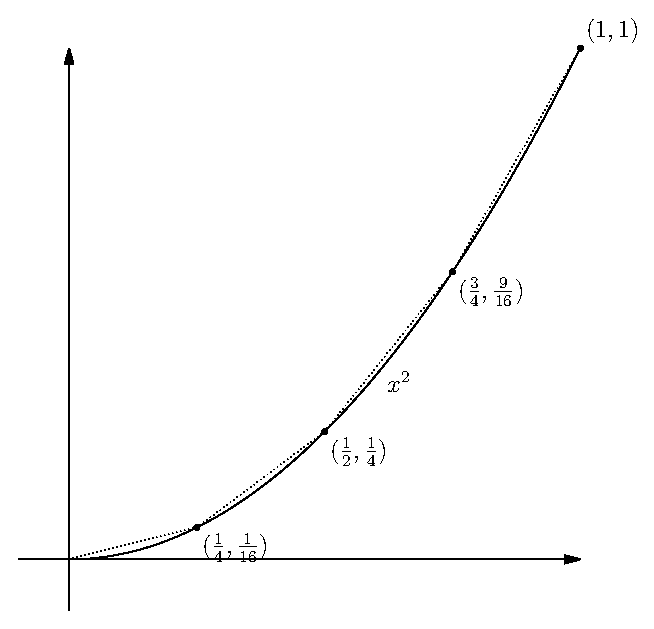
\includegraphics[scale=0.5]{ChapterGeom/Figures/squaredlength_3.eps}
\end{center}
The length is:
$$\sqrt{\left(\frac{1}{4}\right)^2+\left(\frac{1}{16}\right)^2}+\sqrt{\left(\frac{1}{4}\right)^2+\left(\frac{3}{16}\right)^2}+\sqrt{\left(\frac{1}{4}\right)^2+\left(\frac{5}{16}\right)^2}+\sqrt{\left(\frac{1}{4}\right)^2+\left(\frac{7}{16}\right)^2}$$
$$=\frac{1}{16}\left(\sqrt{17}+5+\sqrt{41}+\sqrt{65}\right)\approx1.47$$
}{0in}
\end{itemize}
\end{exercise}

Ok, at this point we get the idea.  More line segments will result in a more accurate approximation, and the limit of these approximations as the number of line segments goes to infinity will produce the exact result.  Here is a \arclength{derivation} that shows this process will result in exactly the right formula.

Let $x_0,x_1,x_2,\ldots,x_n$ be equally spaced points along the $x$-axis from $a$ to $b$.  That is, $x_0=a$, $x_n=b$, and for each $i\in\lbrace 0,1,2,\ldots , n-1 \rbrace$, $\Delta x = x_{i+1}-x_{i}=\frac{b-a}{n}$.

With this setup, if we want the length of a line segment connecting points $x_{i+1}$ and $x_{i}$, we would use the Pythagorean Theorem to obtain: 
$$\sqrt{\left(\Delta x\right)^2+\left(f\left(x_{i+1}\right)-f\left(x_i\right)\right)^2 } $$ as the length.


\begin{align*}
L&=\lim_{n\rightarrow \infty}\sum_{i=0}^{n-1} \sqrt{\left(\Delta x\right)^2+\left(f\left(x_{i+1}\right)-f\left(x_i\right)\right)^2 } \\
&=\lim_{n\rightarrow \infty}\sum_{i=0}^{n-1} \sqrt{1+\frac{\left(f\left(x_{i+1}\right)-f\left(x_i\right)\right)^2}{\left( \Delta x\right)^2} } \sqrt{\left(\Delta x\right)^2} \\
&=\lim_{n\rightarrow \infty}\sum_{i=0}^{n-1} \sqrt{1+\left( \frac{f\left(x_{i+1}\right)-f\left(x_i\right)}{\Delta x}\right)^2 } \Delta x \\
&=\int_{x=a}^{x=b} \sqrt{1+\left( f'(x)\right)^2 } \dif x
\end{align*}

And thus we have our formula for arc length!

\FormulaBox{Arc Length Formula}{
The graph of the function $f(x)$ from $x=a$ to $x=b$ has length $L= \int_{x=a}^{x=b} \sqrt{1+\left( f'(x)\right)^2 } \dif x$.
}

\begin{exercise}{Exact Arc Length of the Parabola \Coffeecup \Coffeecup \Coffeecup}

\begin{itemize}
\item  We now apply this integral formula to calculate the exact length of our parabolic segment.  Plugging in the formula $f(x)=x^2$ into the arc length integral, we obtain:

$$ L= \int_{x=0}^{x=1} \sqrt{1+\left( 2x\right)^2 } \dif x$$

Finish the evaluation of this integral.  ({\bf Hint:}  The \secant{arc length integral} will be quite difficult!  See Example \ref{reappear}.\ref{seccubed} for help.)  

\solushun{\begin{align*}
L&= \int_{x=0}^{x=1} \sqrt{1+\left( 2x\right)^2 } \dif x\\
&=\int_{x=0}^{x=1} \sqrt{1+4x^2 } \dif x\\
&=\int_{x=0}^{x=1} \sqrt{1+4\left(\frac{1}{2}\tan(\theta)\right)^2 }\cdot \frac{1}{2}\sec^2(\theta) \dif x\tag{Let $x=\frac{1}{2}\tan(\theta)$}\\
&=\frac{1}{2}\int_{x=0}^{x=1} \sqrt{\sec^2(\theta)}\cdot \sec^2(\theta) \dif x\\
&=\frac{1}{2}\int_{x=0}^{x=1} \sec^3(\theta) \dif x\\
&=\frac{1}{2}\left[\frac{1}{2}\left(\sec(\theta)\tan(\theta)+\ln|\sec(\theta)+\tan(\theta)|\right)\right]_{x=0}^{x=1}\tag{From \ref{reappear}\ref{seccubed}}\\
&=\frac{1}{4}\left[\left(\sqrt{4x^2+1}2x+\ln|\sqrt{4x^2+1}+2x|\right)\right]_{x=0}^{x=1}\tag{$\tan\theta=2x\implies\tan^2\theta=4x^2\implies\sec^2\theta=4x^2+1$}\\
&=\frac{2\sqrt{5}+\ln|\sqrt{5}+2|}{4}-\left(\frac{2(0)\sqrt{1}+\ln|\sqrt{1}+0|}{4}\right)\\
&=\frac{2\sqrt{5}+\ln|\sqrt{5}+2|}{4}\\
&\approx1.48
\end{align*}}{3in}

\item How does the exact value of the arc length compare to the approximations?
\solushun{The exact value is very close to the approximations, but it is slightly larger than the approximations we used.\\}{0.25in}
\end{itemize}
\AnswerKeyEntry{The exact arc length is $\frac{2\sqrt{5}+\ln\left| 2+\sqrt{5}\right|}{4}$.}
\end{exercise}

\begin{example}{Arc Length of a Hyperbola}\label{HyperBocaBola}

	\begin{wrapfigure}{r}{0.2\textwidth}
    	\centering
		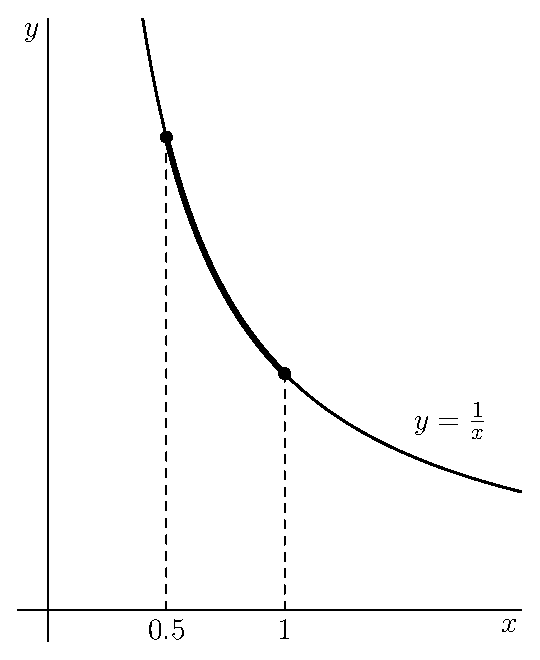
\includegraphics[width=0.2\textwidth]{ChapterGeom/Figures/HyperbolaArcLength}
	\end{wrapfigure}

Suppose we wish to find the arc length $L$ of the hyperbola $$xy=1$$ between the points $\left(\frac{1}{2},2\right)$ and $\left(1,1\right)$.  We begin by solving for the $y$ coordinate in order to express this section of the graph as a function.  Dividing both sides by $x$ produces $$y=f(x)=\frac{1}{x}. $$  We wish to find the length of the graph of this function between $x=\frac{1}{2}$ and $x=1$.  We plug into the arc length formula to obtain $$L= \int_{x=1/2}^{x=1} \sqrt{1+\left( f'(x)\right)^2 } \dif x= \int_{x=1/2}^{x=1} \sqrt{1+\left( -\frac{1}{x^2}\right)^2 } \dif x=\int_{x=1/2}^{x=1} \frac{\sqrt{1+x^4}}{x^2} \dif x. $$ Though we have demonstrated how to set up the arc length integral, it turns out that this integral is quite difficult to evaluate!  In particular, the integrand has no closed form antiderivative.  We will revisit this example in Section \ref{PowerSeriesSubstitution} where we'll have extra tools. 
\end{example}
\begin{exercise}{Checking the Example \Coffeecup}
In the above example...
\begin{itemize}
\item Verify the algebra on the last step, where the integrand is simplified from $\sqrt{1+\left( -\frac{1}{x^2}\right)^2 }$ to $\frac{\sqrt{1+x^4}}{x^2}$. 

\solushun{\begin{align*}
\sqrt{1+\left( -\frac{1}{x^2}\right)^2 }&=\sqrt{1+\frac{1}{x^4} }\\
&=\sqrt{\frac{x^4+1}{x^4} }\\
&=\frac{\sqrt{1+x^4}}{x^2}
\end{align*}}{.5in}

\item Try evaluating the integral via the trigonometric substitution $x=\sqrt{\tan\left(\theta\right)}$.  It may look promising at first!  However, where do you get stuck?

\solushun{\begin{align*}
\int_{x=1/2}^{x=1}\frac{\sqrt{1+x^4}}{x^2}\dif x&=\int\frac{\sqrt{1+\left(\sqrt{\tan\theta}\right)^4}}{\left(\sqrt{\tan\theta}\right)^2}\cdot\frac{\sec^2\theta}{2\sqrt{\tan\theta}}\dif \theta\tag{$x=\sqrt{\tan\theta}$}\\
&=\int_{x=1/2}^{x=1}\frac{\sqrt{1+\tan^2\theta}}{\tan\theta}\cdot\frac{\sec^2\theta}{2\sqrt{\tan\theta}}\dif \theta\\
&=\int_{x=1/2}^{x=1}\frac{\sec^3\theta}{2\left(\tan\theta\right)^{\frac{3}{2}}}\dif \theta\\
&=\frac{1}{2}\int_{x=1/2}^{x=1}\frac{1}{\cos^3\theta\frac{\left(\sin\theta\right)^\frac{3}{2}}{\left(\cos\theta\right)^\frac{3}{2}}}\dif \theta\\
&=\frac{1}{2}\int_{x=1/2}^{x=1}\frac{1}{\left(\cos\theta\sin\theta\right)^\frac{3}{2}}\dif \theta\\
\end{align*}
We get stuck because we don't have a way to evaluate integrals of fractional powers of trig functions.\\}{1in}

\end{itemize}
\end{exercise}
\subsection{Circumference of a Circle }
We now use the arc length integral to compute the \circles{circumference} of a circle.  Though one can take the formula for the circumference of a circle simply as the definition of $\pi$, it is still nice to go through this as proof of concept.  

\begin{exercise}{Circumference of a Circle \Coffeecup \Coffeecup}
\begin{itemize}
\item Use the arc length formula to calculate the circumference of a circle with radius $r$.

\solushun{
Our equation of a circle in terms of $x$ and $r$ can be derived from the standard equation of a circle:
$$x^2+y^2=r^2\implies y=\sqrt{r^2-x^2}$$
Taking the derivative gives $$f'(x)=\frac{-2x}{2\sqrt{r^2-x^2}}=\frac{-x}{\sqrt{r^2-x^2}}$$
To simplify the calculation a bit, we will only find the arc length for the top right quarter of the circle, then multiply the result by $4$.
\begin{align*}
4\int^{x=r}_{x=0}\sqrt{1+\left(f'(x)\right)^2}\dif x&=4\int^{x=r}_{x=0}\sqrt{1+\left(\frac{-x}{\sqrt{r^2-x^2}}\right)^2}\dif x\\
&=4\int^{x=r}_{x=0}\sqrt{1+\frac{x^2}{r^2-x^2}}\dif x\\
&=4\int^{x=r}_{x=0}\sqrt{\frac{r^2-x^2+x^2}{r^2-x^2}}\dif x\\
&=4\int^{x=r}_{x=0}\sqrt{\frac{r^2}{r^2-x^2}}\dif x\\
&=4r\int^{x=r}_{x=0}\sqrt{\frac{1}{r^2-x^2}}\dif x\\
&=4r\int^{\theta=\pi/2}_{\theta=0}\sqrt{\frac{1}{r^2-\left(r\sin(\theta)\right)^2}}\cdot r\cos(\theta)\dif \theta\tag{Let $x=r\sin(\theta)$}\\
&=4r\int^{\theta=\pi/2}_{\theta=0}\frac{r\cos(\theta)}{r\cos(\theta)} \dif \theta\tag{Let $x=r\sin(\theta)$}\\
&=4r\left[\theta\right]^{\pi/2}_{0}\\
&=4r\left[\frac{\pi}{2}-0\right]\\
&=2\pi r\\
\end{align*}}{2in}

\item Take the derivative of your formula for area of a circle with respect to $r$.  How does it relate to your formula for the circumference of a circle?  Draw a picture and indicate why this freakish coincidence actually geometrically makes sense.

\solushun{$$\dfrac{\dif}{\dif r}\pi r^2=2\pi r$$
The derivative of the equation for area of a circle is the same  as the equation for the circumference of a circle. The definition of the derivative suggests that the derivative the area of a circle of radius $r$ is the limit of the difference between that circle and a slightly larger circle of radius $r+\Delta r$ as $\Delta r$ approaches 0. This can be visualized as cutting out the smaller circle from the larger one, and investigating what happens as the larger circle approaches the size of the smaller one.
\begin{center}
$$\dfrac{\dif}{\dif r}\pi r^2=\lim_{\Delta r\to0}\frac{\pi (r+\Delta r)^2-\pi r^2}{\Delta r}=\pi\lim_{\Delta r\to0}\frac{r^2+2r\Delta r+\Delta r^2- r^2}{\Delta r}=\pi\lim_{\Delta r\to0}2r+\Delta r=2\pi r$$
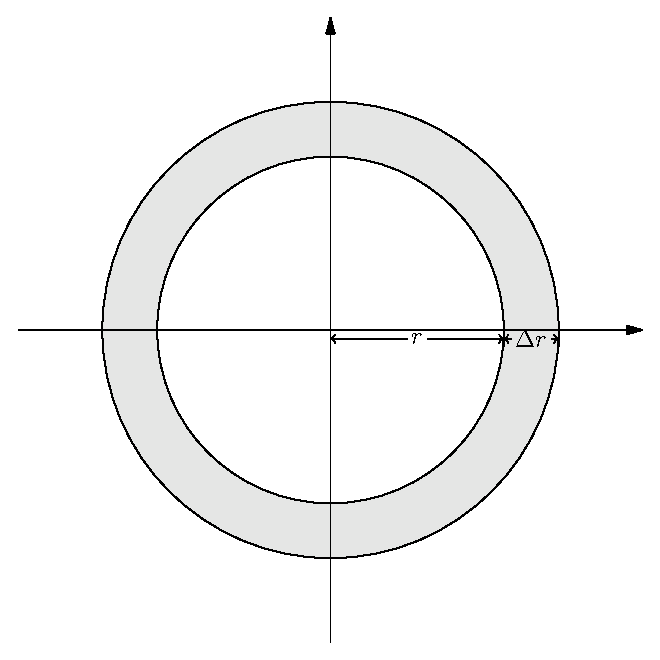
\includegraphics[scale=0.5]{ChapterGeom/Figures/circderiv.eps}
\end{center}}{1in}
\end{itemize}
\end{exercise}

\subsection{Lengths of Some Other Fun Arcs}
\begin{exercise}{Other Arcs \Coffeecup \Coffeecup \Coffeecup}

Draw the graph and compute the length of each of the following arcs using our arc length formula.
\begin{itemize}
\item Line segment from a point $(x_0,y_0)$ to a point $(x_1,y_1) $.  ({\bf Hint:} To get your function, use the point-slope form of a line and then solve for $y$.)  How does this compare to the length the Pythagorean Theorem would give you?

\solushun{
\begin{center}
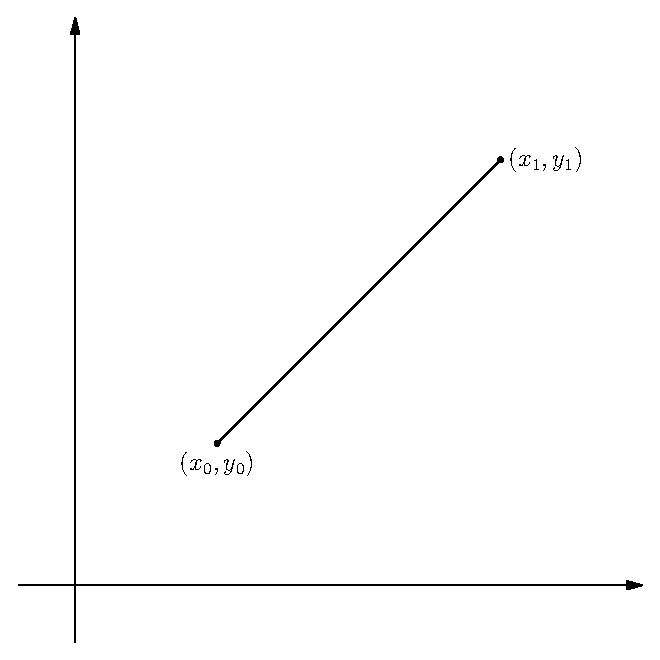
\includegraphics[scale=1]{ChapterGeom/Figures/linearc.eps}
\end{center}
$$(y-y_1)=m(x-x_1)\implies y=\frac{y_1-y_0}{x_1-x_0}x+y_1=f(x)$$
$$f'(x)=\frac{y_1-y_0}{x_1-x_0}$$
\begin{align*}
\int^{x_1}_{x_0}\sqrt{1+\left(\frac{y_1-y_0}{x_1-x_0}\right)^2}\dif x&=\sqrt{1+\left(\frac{y_1-y_0}{x_1-x_0}\right)^2}\left.x\right|^{x_1}_{x_0}\\
&=\sqrt{\frac{(x_1-x_0)^2+(y_1-y_0)^2}{(x_1-x_0)^2}}\left(x_1-x_0\right)\\
&=\frac{\sqrt{(x_1-x_0)^2+(y_1-y_0)^2}}{(x_1-x_0)^2}\left(x_1-x_0\right)\\
&=\sqrt{(x_1-x_0)^2+(y_1-y_0)^2}
\end{align*}
This is what we would get from the Pythagorean Theorem.\\}{2in}

\item The graph of $f(x)=\ln(x)$ from $x=1$ to $x=e$.  Take an approximation using two line segments, and then get the exact length using an arc length integral.  How do they compare?

\solushun{
\begin{center}
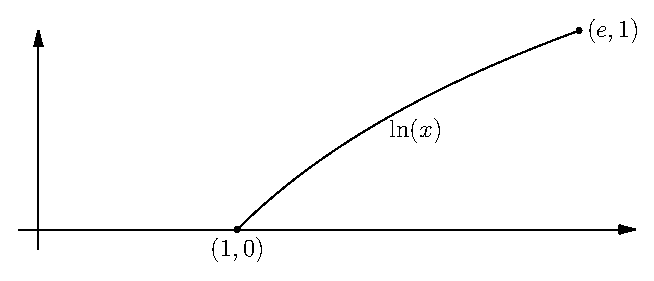
\includegraphics[scale=1]{ChapterGeom/Figures/lnarc.eps}
\end{center}
\begin{align*}
\int^e_1\sqrt{1+\left(\frac{1}{x}\right)^2}\dif x &= \int^e_1\sqrt{\frac{x^2+1}{x^2}}\dif x\\
\text{Let } x=\tan(\theta), \dif x=\sec^2(\theta)\dif\theta. \text{Then: }\\
\int^e_1\sqrt{\frac{x^2+1}{x^2}}\dif x&=\int^{x=e}_{x=1}\sqrt{\frac{\tan^2(\theta)+1}{\tan^2(\theta)}}\sec^2(\theta)\dif\theta\\
&=\int^{x=e}_{x=1}\frac{\sec^3(\theta)}{\tan(\theta)}\dif\theta\\
&=\int^{x=e}_{x=1}\sec^2(\theta)\csc(\theta)\dif\theta\\
\text{Now via IBP, let }\\
u=\csc(\theta), \dif u=-\csc(\theta)\cot(\theta), \\
v=\tan(\theta), \dif v =\sec^2(\theta)\\
\int^{x=e}_{x=1}\sec^2(\theta)\csc(\theta)\dif\theta&=\csc(\theta)\tan(\theta)+\int^{x=e}_{x=1}\tan(\theta)\csc(\theta)\cot(\theta)\dif\theta\\
&=\csc(\theta)\tan(\theta)+\int^{x=e}_{x=1}\csc(\theta)\dif\theta\\
&=\csc(\theta)\tan(\theta)-\ln\left|\csc(\theta)+\cot(\theta)\right|^{x=e}_{x=1}\\
\text{Draw a triangle to see that }\\
\csc(\theta)=\frac{\sqrt{x^2+1}}{x}\\
\tan(\theta)=x\\
\cot(\theta)=\frac{1}{x}\\
\text{Then: }\\
\csc(\theta)\tan(\theta)-\ln\left|\csc(\theta)+\cot(\theta)\right|^{x=e}_{x=1}&=\sqrt{x^2+1}-\ln\left|\frac{\sqrt{x^2+1}+1}{x}\right|^{x=e}_{x=1}\\
&=\left.\sqrt{x^2+1}-\ln\left|\sqrt{x^2+1}+1\right|-\ln|x|\right|^{x=e}_{x=1}\\
&=\sqrt{e^2+1}-\ln\left|\sqrt{e^2+1}+1\right|-\ln|e|-\left(\sqrt{1+1}-\ln\left|\sqrt{1+1}+1\right|-\ln|1|\right)\\
&=\sqrt{e^2+1}-\ln\left|\sqrt{e^2+1}+1\right|-1-\sqrt{2}+\ln\left|\sqrt{2}+1\right|\\
&\approx 2.003497
\end{align*}
To make the integral look like the nice symmetrical answer in the answer key requires some manipulation:
\begin{align*}
\sqrt{x^2+1}-\ln\left|\frac{\sqrt{x^2+1}+1}{x}\right|&=\sqrt{x^2+1}+\ln\left|\frac{x}{\sqrt{x^2+1}+1}\right|\\
&=\sqrt{x^2+1}+\frac{1}{2}\ln\left|\frac{x^2}{\left(\sqrt{x^2+1}+1\right)^2}\right|\\
&=\sqrt{x^2+1}+\ln\left|\frac{x^2+1-1}{\left(\sqrt{x^2+1}+1\right)^2}\right|\\
&=\sqrt{x^2+1}+\ln\left|\frac{\sqrt{x^2+1}^2-1^2}{\left(\sqrt{x^2+1}+1\right)^2}\right|\\
&=\sqrt{x^2+1}+\ln\left|\frac{\left(\sqrt{x^2+1}-1\right)\left(\sqrt{x^2+1}+1\right)}{\left(\sqrt{x^2+1}+1\right)^2}\right|\\
&=\sqrt{x^2+1}+\ln\left|\frac{\sqrt{x^2+1}-1}{\sqrt{x^2+1}+1}\right|
\end{align*}
}{3in}

\item The graph of $f(x)=e^x$ from $x=0$ to $x=1$.

\solushun{
Since the natural logarithm is the inverse of the natural exponential function, the length of the arc from corresponding segments will be the same. In this case, that's exactly what we have, since $\ln(1)=0, \ln(e)=1$.

So the arc length of $e^x$ from $x=0$ to $x=1$ is also approximately 2.003497.

To be precise, we could use the same formula we got above, and just set our bounds to be the value of the exponential at the endpoints of our range. That is, the arc length of $e^x$ from $x=a$ to $x=b$ with $b>a$ is:
$$\left[\sqrt{x^2+1}+\ln\left|\frac{\sqrt{x^2+1}-1}{\sqrt{x^2+1}+1}\right|\right]^{e^b}_{e^b}$$
Actually calculating the integral reveals an interesting connection between the two.
$$\int\sqrt{1+e^{2x}}\dif x = \sqrt{1+e^{2x}}+1+\ln\left|\frac{e^{2x}}{\sqrt{1+e^{2x}}+1}\right|+C$$
The actual process involves 3 rounds of $u$-substitutions. This is a good example of where clever use of previous results can save you a lot of time and effort.\\
}{1in}

%KHALED: I need to check and confirm that last integral of the arc length of e^x

\end{itemize}

\AnswerKeyEntry{The length of the graph of the natural logarithm from (1,0) to (e,1) is $$\sqrt{e^2+1}+\frac{1}{2}\ln\left| \frac{\sqrt{e^2+1}-1}{\sqrt{e^2+1}+1}\right|-\sqrt{2}+\frac{1}{2}\ln\left| \frac{\sqrt{2}+1}{\sqrt{2}-1}\right| $$ which is roughly 2.003497.  Also, notice that the natural exponential function is just the inverse of the natural logarithm; think about what this means regarding arc length!}
\end{exercise}

\subsection{Surface Area}

For the \integ{surface area} of a surface of revolution, we use the \surfacearea{frustum of a right circular cone} as the object that approximates the surface, much as we used line segments for arc length.  Thus, to get off the ground, we must figure out what the \cone{surface area of a frustum} is.  Suppose it has inner radius $r$ and outer radius $R$ and let $L$ be the diagonal length, top to bottom, of the frustum.  Project the shape onto a flat plane sitting under it to produce a washer whose outer radius is $R$ and inner radius is $r$.

	\begin{center}
		\includegraphics[width=300pt]{ChapterGeom/Figures/frustraproj.eps}
	\end{center} 

Notice that the washer in the plane has area $\pi (R^2-r^2)$.  Also, the radial lengths got uniformly scaled by a factor of $\frac{L}{R-r}$, since every segment of length $R-r$ got stretched into a segment of length $L$.  Thus we have that the area of the frustum is $\frac{L}{R-r}\cdot \pi (R^2-r^2)$, which simplifies to: $$SA=\pi L (R+r) $$

\begin{exercise}{\parabola{Surface Area of a Paraboloid} \Coffeecup \Coffeecup \Coffeecup}
To test this out, consider the parabola $y=x^2$ from $x=0$ to $x=1$.  Create a surface by revolving this curve around the $y$-axis.  
\begin{itemize}
\item Approximate the surface area of this region using two frusta, one that goes from $x=0$ to $x=1/2$, and one that goes from $x=1/2$ to $x=1$.

	\begin{center}
		\includegraphics[width=300pt]{ChapterGeom/Figures/parabfrustrum.eps}
	\end{center} 

\solushun{
To get $L_1$ the length of the first frustrum, we need to find the length of the segment from $(0,0)$ to $(\frac{1}{2},\frac{1}{4})$.
$$L_1 = \sqrt{\frac{1}{4}+\frac{1}{16}} = \frac{\sqrt{5}}{4}$$
Similarly, $L_2$, the length of the second frustrum is:
$$L_2 = \sqrt{\frac{1}{4}+\frac{9}{16}} = \frac{\sqrt{13}}{4}$$
$r_1=0$ because it is the inner radius of the bottom cone, which is actually closed at the origin, and $R_1=\frac{1}{2}$. $r_2=\frac{1}{2}$ and $R_2=1$.
Now we have everything we need to estimate our surface area.
\begin{align*}
SA=\pi L_1(r_1+R_1)+\pi L_2(r_2+R_2)&=\pi\left(\frac{\sqrt{5}}{4}\left(\frac{1}{2}\right)+ \frac{\sqrt{13}}{4}\left(\frac{1}{2}+1\right)\right)\\
&=\pi\left(\frac{\sqrt{5}}{8}+ \frac{3\sqrt{13}}{8}\right)\\
&=\frac{\pi}{8}\left(\sqrt{5}+3\sqrt{13}\right)\\
&\approx 5.126
\end{align*}
}{1in}

\item As in the previous cases, we can see that chopping it up into more approximating regions will increase the accuracy of our approximation as the number of these goes to infinity.  However, actually adding up the surface areas by hand would become frusta-ting, so instead we just set up a limit of a summation.  Draw a diagram and set up the limit of a sum of surface areas of frusta, similarly to how we did for the arc length formula.  Fill in the middle part of the derivation below:


\begin{align*}
L&=\lim_{n\rightarrow \infty}\sum_{i=0}^{n-1} \pi\sqrt{\left(x_{i+1}-x_i\right)^2+\left(f(x_{i+1})-f(x_i)\right)^2}\left(x_{i+1}+x_{i} \right)  \\
&=  \\
&= \\
&= \\
&= \\
&= \\
&=\int_{x=a}^{x=b} 2 \pi x \sqrt{1+\left(f'(x)\right)^2} \dif x \\
\end{align*}

\solushun{
\begin{align*}
L&=\lim_{n\rightarrow \infty}\sum_{i=0}^{n-1} \pi\sqrt{\left(x_{i+1}-x_i\right)^2+\left(f(x_{i+1})-f(x_i)\right)^2}\left(x_{i+1}+x_{i} \right)  \\
&= \lim_{n\rightarrow \infty}\sum_{i=0}^{n-1} \pi\sqrt{1+\left(\frac{f(x_{i+1})-f(x_i)}{x_{i+1}-x_i}\right)^2}\left(x_{i+1}+x_{i} \right) \\
&= \lim_{n\rightarrow \infty}\sum_{i=0}^{n-1} \pi\sqrt{1+\left(\frac{f(x_{i+1})-f(x_i)}{x_{i+1}-x_i}\right)^2}\left(x_{i}+\Delta x+x_{i} \right) \\
&= \lim_{n\rightarrow \infty}\sum_{i=0}^{n-1} \pi\sqrt{1+\left(\frac{f(x_{i+1})-f(x_i)}{x_{i+1}-x_i}\right)^2}(2x_i+\Delta x) \\
&=\int_{x=a}^{x=b} 2 \pi x \sqrt{1+\left(f'(x)\right)^2} \dif x \\
\end{align*}
        Note: to get from the 3rd to the 4th step, remember that as the number of subdivisions of the interval along the $x$-axis from the start point to the end point approaches infinity, the difference between each $x_i$ approaches 0. We can call this difference $\Delta x$ and note that $x_{i+1}=x_i+\Delta x$. If this $\Delta x$ goes to 0, it makes some sense that $\lim_{n\to\infty}(x_{i+1}+x_i)=(2x_i)$ plus the differential $\dif x$.\\
}{0in}

\item Use this integration formula to find the exact surface area of the parabolic bowl.  How does it compare to your approximation?

\solushun{
\begin{align*}
L &= \int_0^1 2\pi x\sqrt[]{1+((x^2)')^2} \dif x \\
&= 2\pi \int_0^1 x\sqrt[]{1+((2x)')^2} \dif x \\
&= 2\pi \int_0^1 x\sqrt[]{1+4x^2} \dif x \\
\text{Via trig sub:}\\
x = \frac{1}{2}\tan\theta \\
\dif x = \frac{1}{2}\sec^2\theta \dif \theta \\
&= 2\pi \int_{x=0}^{x=1} \frac{1}{2}\tan\theta \sqrt[]{1+\tan^2\theta} \frac{1}{2}\sec^2\theta \dif \theta \\
&= \frac{1}{2} \pi \int_{x=0}^{x=1} \tan\theta\sec^3\theta \dif\theta \\
\text{Let }u=\sec \theta , \; \dif u= \tan\theta \sec\theta \dif \theta \\
&= \frac{1}{2} \pi \int_{x=0}^{x=1} u^2 \dif u \\
&= \left. \frac{1}{2} \frac{u^3}{3} \right|_{x=0}^{x=1} \\
&= \left. \frac{1}{6}\pi \sec^3\theta \right|_{x=0}^{x=1} \\
\text{Draw a triangle to see that:}\\
\sec\theta = \sqrt[]{1+4x^2}\\
&= \left. \frac{1}{6}\pi \left(\sqrt[]{1+4x^2} \right)^3 \right|_{x=0}^{x=1}\\
&= \frac{\pi}{6}\left(\sqrt[]{5}\right)^3-\frac{\pi}{6} \\
&\approx 5.3304
\end{align*}
We see that this answer is slightly bigger than the approximation, which is to be expected.
}{0in}

\end{itemize}
\AnswerKeyEntry{The two-frusta approximation is $$\frac{\pi}{8}\left(\sqrt{5}+3\sqrt{13} \right)\approx 5.126 $$  The exact value of the surface area is $$\frac{\pi}{6}\left(5\sqrt{5}-1 \right)\approx 5.3304 $$ which is just slightly larger, as one would expect. }
\end{exercise}

\begin{exercise}{\sphere{Surface Area} of a \surfacearea{Sphere} \Coffeecup \Coffeecup}

Notice that a sphere is a surface of revolution created by a circle centered at the origin.  Since the right-hand side of a circle is not the graph of a function, we will just use the top right quarter circle to revolve about the $y$-axis and then multiply by 2 to pick up the bottom half of the sphere.  
\begin{itemize}
\item In particular, use the function $f(x)=\sqrt{r^2-x^2}$ for $x=0$ to $x=r$ in our surface area integral to find the formula for the surface area for a sphere of radius $r$.

\solushun{
If $f(x)=\sqrt{r^2-x^2}$, $f'(x)=-\frac{x}{\sqrt{r^2-x^2}}$. Then the integral is set up as:
\begin{align*}
\int_0^r2\pi x\sqrt{1+\left(-\frac{x}{\sqrt{r^2-x^2}}\right)^2}\dif x&=\int_0^r2\pi x\sqrt{1+\left(\frac{x^2}{r^2-x^2}\right)}\dif x\\
&=2\pi \int_0^rx\sqrt{\frac{r^2-x^2+x^2}{r^2-x^2}}\dif x\\
&=2\pi \int_0^rx\sqrt{\frac{r^2}{r^2-x^2}}\dif x\\
&=2\pi r\int_0^rx\frac{1}{\sqrt{r^2-x^2}}\dif x\\
\text{Let $u=r^2-x^2, \dif u=-2x \dif u$}\\
&=2\pi r\cdot -\frac{1}{2}\int_0^r\frac{1}{\sqrt{u}}\dif u\\
&=-\pi r\left[2u^{\frac{1}{2}}\right]_{x=0}^{x=r}\\
&=-2\pi r\left[\sqrt{r^2-x^2}\right]_{x=0}^{x=r}\\
&=-2\pi r\left[\sqrt{r^2-r^2}-\sqrt{r^2}\right]\\
&=-2\pi r\left[-r\right]\\
&=2\pi r^2\\
\end{align*}
To get the total sphere, we double this to $4\pi r^2$.\\
}{2in}

\item Take the derivative of the formula for sphere volume with respect to $r$. How
does it relate to the formula for surface area? Again, draw a diagram explaining
this geometrically.

\solushun{The derivative of volume with respect to $r$ is:
$$\dfrac{\dif}{\dif r}\frac{4}{3}\pi r^3=4\pi r^2$$
This is the formula we just got for the surface area of a sphere. Similar to the relationship between the derivative of area and the circumference of a circle, this shows how the volume of a sphere approaches its surface area as the difference, or range, of its radius approaches 0. This can be conceptualized as a sphere with a region inside it that is hollow. When the sphere is solid, the inner region's radius is 0. As the difference between the inner region's radius and the sphere's radius approaches 0, the sphere becomes a hollow ball.\\}{2in}

\end{itemize}
\end{exercise}

\subsection{Volume}\label{Volume}

We have two fundamentally different methods for computing volume: \integ{volume by cross sections} and volume by cylindrical shells.

\subsubsection{Volume by Cross-sectional Area}

Recall that we calculate the area of a planar region by integrating the height at each $x$-coordinate; here we compute volume of a 3D solid by integrating the area at each $x$-coordinate.  More formally, we say that the volume of a 3D figure that starts at $x = a$ and ends at $x = b$ with the function $A(x)$ representing the area of the cross-section at
coordinate $x$ is given by the integral of the cross-sectional areas.

\FormulaBox{Volume Equals the Integral of Cross Sectional Area}{
The volume of the solid from $x=a$ to $x=b$ with cross-sectional area $A(x)$ is $V= \int_{x=a}^{x=b} A(x) \dif x$. 
}
 
\subsubsection{The Cone, Pyramid, and Tetrahedron}
Let's try this out on a cone!  Suppose we have a right circular cone of height $h$ and radius $r$.  Place the cone so that the vertex lies at the origin and the center of the base lies at the point $(h,0,0)$. 

	\begin{center}
		\includegraphics[width=300pt]{ChapterGeom/Figures/Cone.eps}
	\end{center}


Any cross section parallel to the base is clearly a circle.  Thus to compute the area of each circle we just need to find the radius of an arbitrary cross section at location $x$.  To help us, we imagine a 2D ``side view'' of the middle of the \volume{cone}.

	\begin{center}
		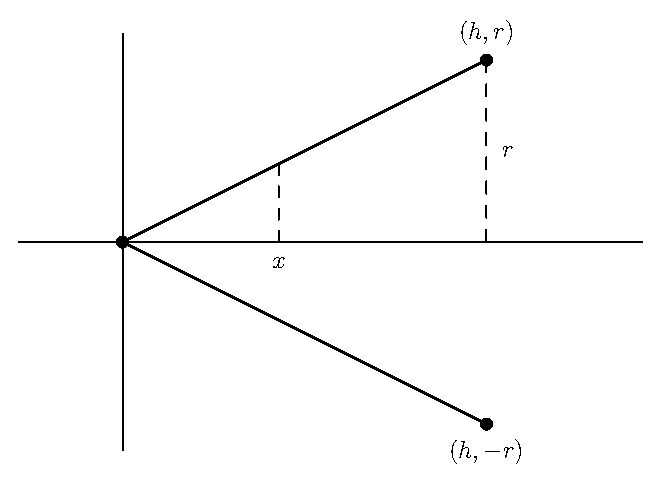
\includegraphics[width=300pt]{ChapterGeom/Figures/conetriangle.eps}
	\end{center} 

Notice the top boundary of this shape is the graph of the linear function $f(x)=\frac{r}{h}x$.  This height is exactly the radius of the circular cross section of the cone at location $x$. 
\begin{exercise}{Check the Boundary \Coffeecup}
  Briefly explain why this formula is the correct formula for the top boundary!
\solushun{Since the height is $h$ and the run is $r$, we have a slope of $\frac{h}{r}$. Thus, the line $f(x)=\frac{h}{r}x$ describes the boundary.\\}{1in}
\end{exercise}
\begin{example}{Volume of a Cone by Cross Sections}
We can now set up and evaluate our \cone{volume} integral. \begin{align*}
V&=\int_{x=0}^{x=h}A(x) \dif x \\
&= \int_{x=0}^{x=h}\pi \left(\frac{r}{h}x\right)^2 \dif x \\
&= \int_{x=0}^{x=h}\pi \frac{r^2}{h^2}x^2 \dif x \\
&= \left.\pi \frac{r^2}{3h^2}x^3 \right|_{x=0}^{x=h} \\
&= \pi \frac{r^2}{3h^2}h^3 -0 \\
&= \frac{1}{3}\pi r^2 h
\end{align*}

\end{example}

Note that this is actually a very clean formula; it says the area of a cone is one-third times the area of the base times the height.
\begin{exercise}{The Pyramid \Coffeecup \Coffeecup }
\begin{itemize} \item Consider a square base pyramid of side length $s$ and height $h$.  What would you conjecture for the volume of this solid based on our cone computation above?
\solushun{Conjecture that $V = \frac{1}{3}hr^2$.\\}{.5in}

	\begin{center}
		\includegraphics[width=300pt]{ChapterGeom/Figures/pyramid.eps}
	\end{center} 

\item Use integration of cross sectional area to verify your conjecture and formally compute the volume of the pyramid.

\solushun{
Based on the diagram, consider your function to be $f(x) = \frac{r}{2h}x\cdot \frac{r}{h}x$. Proceeding:
\begin{align*}
V &= \int_{x=0}^{x=h} \frac{r^2}{2h^2}x^2 \dif x \\
&= \left. \frac{r^2}{6h^2}x^3\right|_{x=0}^{x=h} \\
&= \frac{r^2}{6h^2}h^3\\
&= \frac{r^2h}{3}\\
&= \frac{1}{3}hr^2
\end{align*}
Which we see is the same as our conjecture.\\
}{0in}
%KHALED: Need to learn how to make 3d asymptote images...weekend project

\end{itemize}
\AnswerKeyEntry{Notice that if you turn the pyramid sideways, you can get the 2D side view to be almost exactly the same as we had for the cone!  The volume is $V=\frac{1}{3}r^2h$.}
\end{exercise}

\begin{exercise}{A Tetrahedron \Coffeecup \Coffeecup}
 \begin{itemize} \item In three dimensions, plot a tetrahedron that has vertices $(0,0,0), (a,0,0), (0,b,0),$ and $(0,0,c)$.  Based on how the volumes came out for the cone and pyramid, what would you suspect for the \tetrahedron{volume} of this figure?

\solushun{We would expect it to be $\frac{1}{3}$ the base times the height. With a base of $\frac{1}{2}ab$ and a height of $c$, that gives $\frac{1}{6}abc$.\\}{1in}

\item Use integration of cross sections to find the volume of that tetrahedron.
\solushun{
Each edge of the tetrahedron is described by a line, one with slope $-\frac{c}{a}$, one with slope $-\frac{b}{a}$, and one with slope $-\frac{c}{b}$, we can slice the volume perpendicular to the $x$-axis. Then the height of each cross section is $-\frac{c}{a}x$ and the width is $-\frac{b}{a}x$. Each cross section is a triangle, so our function for the area of the cross section is $f(x) = \left(-\frac{c}{a} \cdot -\frac{b}{a}x \right)\frac{1}{2}$. Proceeding:
\begin{align*}
V &= \frac{1}{2} \int_{x=0}^{x=a} \frac{bc}{a^2}x^2 \dif x \\
&= \left. \frac{1}{2} \cdot \frac{bc}{a^2}x^3 \right|_{x=0}^{x=a} \\
&= \frac{a^3bc}{6a^2}\\
&= \frac{1}{6}abc=\frac{1}{3}\cdot\frac{1}{2}abc
\end{align*}
Interestingly, a tetrahedron with $a=b$ is a quarter of a square pyramid, where $r=\sqrt{a^2+b^2}=\sqrt{2a^2}$. As such, we should expect it to have a volume of $\frac{1}{4}$ the volume of the pyramid, or $\frac{1}{12}r^2h=\frac{1}{12}2a^2c=\frac{1}{6}a^2c$. So a pyramid can be seen as a special case of a set of 4 tetrahedrons, all with base edges of the same length, set next to each other.\\
}{1in}
\end{itemize}
\AnswerKeyEntry{The volume is $V=\frac{1}{6}abc$.}
\end{exercise}

\begin{exercise}{Other Bases \Coffeecup \Coffeecup \Coffeecup \Coffeecup}
\begin{itemize}
\item What happens if you start with other shapes as the base of your figure?  If you form a solid by connecting the boundary of the base to a point with line segments, do you always get just one-third times the area of the base times the height as the volume?  Or, can you find some bases for which this formula does not hold?
\solushun{No matter the shape of the base, the volume will always be $\frac{1}{3}$ times the area of the base times the height. This is because when we integrate any of these volumes, we can always integrate along the $x$-axis, with the base arranged perpendicular to the $x$-axis. Since the area of any given cut is dependent on $x$ and is an area, it should be expressible with a squared power of $x$, which when integrated gives us a $\frac{1}{3}$ Since the slope of the lines connecting the base to the vertex is dependent on the height (that is, $\frac{b}{h}$ where $b$ is some defining measure of the base and $h$ is the height of the ``cone''), we will always end up with something like the following:
$$
\int_0^h a\frac{b^2}{h^2}x^2\dif x=\left.a\frac{b^2}{h^2}\cdot\frac{x^3}{3}\right|^h_0=\frac{1}{3}ab^2h
$$
Where $a, c$ constants. In our cone, $a=\pi$ and $c=r$. In the pyramid $a=\frac{1}{2}$ and $c=r$.
Thus, as long as we can express the area of the base with some function of the form $A(b)=ab^2$, we will see the pattern.

Even odd shapes, such as a circular cone with a cut in it or a knob sticking out could be expressed as the sum or difference of shapes that fit the model (though calculating overlapping areas might be tricky).\\

%A parabolic cone, where the base is a parabola cut at the height equal to half its width will present an interesting puzzle, since to ensure its height is actually always equal to half its width requires changing the parabolas function's coefficient as you extend the cone (otherwise the slope of the edge of the cone will not be a straight line). But even in this case, the pattern holds.\\
}{3in}
\end{itemize}
\end{exercise}

\subsubsection{The Sphere}

A sphere of radius $r$ is a solid of revolution constructed by rotating a circle of radius $r$ centered at the origin about either the $x$ or $y$ axis.  First, we use cross-sectional area, which many sources call the ``disc method" since a cross-section of a \volume{sphere} is a circular disc.  

	\begin{center}
		\includegraphics[width=300pt]{ChapterGeom/Figures/spherebydisks.eps}
	\end{center} 

\begin{exercise}{The \sphere{Volume} of a Sphere \Coffeecup \Coffeecup}
\begin{itemize} \item Draw a 2D ``side view'' of the sphere much like we did for the cone.  What is the formula for the top boundary curve? 

\solushun{
$$y=\sqrt{r^2-x^2}$$
}{1in}

\item Compute the volume of a sphere via an integral of cross-sectional area.

\solushun{
Each slice is a circle of radius $r$ equal to $y=\sqrt{r^2-x^2}$. The area of each slice is therefore $A(x)=\pi r^2=\pi\left(\sqrt{r^2-x^2}\right)^2$.
\begin{align*}
\int_{-r}^r\pi\left(\sqrt{r^2-x^2}\right)^2\dif x&=\pi\int_{-r}^r r^2-x^2\dif x\\
&=\pi \left[r^2x-\frac{x^3}{3}\right]_{-r}^r\\
&=\pi \left[r^3-\frac{r^3}{3}-\left(-r^3-\frac{-r^3}{3}\right)\right]\\
&=\pi \left[2r^3-\frac{2r^3}{3}\right]\\
&=\frac{4}{3}\pi r^3
\end{align*}}{2in}

\end{itemize}
\AnswerKeyEntry{The circular cross section has equation $x^2+y^2=1$.  If you solve for the $y$ coordinate, you'll have a function for the radius of a circular cross section at position $x$.  This formula can be integrated to produce the volume $V=\frac{4}{3}\pi r^3$.}
\end{exercise}

It is worth noting that this process works equally well if we slice along the $y$-axis instead of the $x$-axis.  

\begin{example}{Volume of a Parabolic Bowl (Para-bowl-a?)}
Consider the region bounded by $y=x^2, y=0,x=0$, and $x=1$.  Revolve this 2D region about the $y$-axis to create a bowl.  This would be an absolute mess to examine via cross sections in the $x$ direction, since they do not have an easily describable shape.  However, in the $y$ direction, the cross sections are all just circles with smaller circles deleted.  Specifically, at height $y$, we have a circle of radius 1 with a circle of radius $x=\sqrt{y}$ deleted from it.  Thus, the area of the cross section at height $y$ is given by $$A(y)=\pi\cdot 1^2-\pi \cdot \left(\sqrt{y}\right)^2 $$ for $y=0$ to $y=1$. 
\end{example}

This case, where cross-sections are large circles with small circles deleted, occurs fairly frequently.  Many references call this the \emph{washer method}, though it is really just a special case of cross sections.
 
\begin{exercise}{Finish the Example \Coffeecup}\label{ParaBowla}
\begin{itemize}\item Find the volume of the parabolic bowl described above by evaluating the integral $$V=\int_{y=0}^{y=1}A(y)\dif y. $$
\solushun{
\begin{align*}
V=\int_{y=0}^{y=1}\pi-\pi\left(\sqrt{y}\right)^2\dif y&=\pi\int_{y=0}^{y=1}1-y\dif y\\
&=\pi\left[y-\frac{y^2}{2}\right]_{0}^{1}\\
&=\pi\left[1-\frac{1}{2}\right]\\
&=\frac{\pi}{2}
\end{align*}}{1in}

\item Consider the cylinder centered at the $y$-axis with height 1 and radius 1.  What percent of the volume of that cylinder is occupied by the parabolic bowl? 

\solushun{
The volume of the cylinder is $V_c=\pi\cdot1^2\cdot1=\pi$. The bowl occupies half of that, so 50\% of the volume of the cylinder is occupied by the bowl.\\
}{.5in}

\end{itemize}
\AnswerKeyEntry{The parabolic bowl has volume $\pi/2$ and occupies exactly fifty percent of the cylinder it sits in!}
\end{exercise}

\subsubsection{Cylindrical Shells}

Another technique that could have been used to compute the volume of the \volume{sphere} is \integ{volume by cylindrical shells}. Let $R$ be a region bounded by $x=a$ and $x=b$ on the sides and bounded by $f(x)$ and $g(x)$ above and below respectively.  Let $S$ be the solid generated by revolving $R$ about the $y$-axis.  The volume of $S$ is as follows:   \FormulaBox{Volume by Cylindrical Shells about $y$-axis}{The volume of $S$ is $V=2\pi \displaystyle\int_{x=a}^{x=b} x\left(f(x)-g(x)\right) \dif x$.}



This formula comes from approximating the volume of the region by using nested cylinders with smaller cylinders deleted from their middle (hence \emph{cylindrical shells}).  In particular, we are cutting the region into shells that approximate the volume, and then taking the limit as the thickness of these shells goes to zero (and the number of shells goes to infinity). 

\begin{definition}{Cylindrical Shells}
 A \emph{cylindrical shell} is a cylinder with a second cylinder of equal height but smaller radius deleted out of the middle of it.
\end{definition}

	\begin{center}
		\includegraphics[width=300pt]{ChapterGeom/Figures/cylinder.eps}
	\end{center} 

\begin{exercise}{The Volume of a Single Cylindrical Shell \Coffeecup }\label{SingleShell}
  See the diagram above of a cylindrical shell with height $h$, outer radius of $r_2$, and inner radius $r_1$.  Show the volume of that shell is given by $V=h\pi\left( r_2^2-r_1^2\right)$.
\solushun{
The volume of the inner shell if $V_1=\pi r_1^2h$ and the outer shell is $V_2=\pi r_2^2h$. Then, their difference $V$ is:
$$V=V_2-V_1=\pi r_2^2h-\pi r_1^2h=h\pi\left( r_2^2-r_1^2\right)$$
}{1in}

\end{exercise}

We test this new method out on a familiar object, the sphere!  

\begin{exercise}{\sphere{Volume} of a Sphere, Again! \Coffeecup \Coffeecup} Suppose we have a sphere of radius $1$.  \begin{itemize} \item To start, approximate the volume of a sphere in a very crude manner.  Obtain an upper bound for the volume by enclosing the sphere in just a single cylinder of height $2$ and radius $1$.

\solushun{
	$$V=\pi r^2 h = \pi \cdot (1)^2 \cdot 2 = 2\pi$$
}{1in}

\item To get a better estimate, we now approximate the volume using six shells.  In the diagram below, assume the center of the sphere is the origin.  Then label the points with $x$-coordinates $x_0=0,x_1=\frac{1}{6},x_2=\frac{2}{6},x_3=\frac{3}{6},x_4=\frac{4}{6},x_5=\frac{5}{6},$ and $x_6=1$.
Compute the volume of each cylindrical shell using the formula from Exercise \ref{Volume}.\ref{SingleShell}.  Add those six volumes to estimate the volume of the sphere.
Label the points and corresponding shell volumes in the diagram below.

	\begin{center}
		\includegraphics[width=300pt]{ChapterGeom/Figures/circleshells.eps}
	\end{center} 

\item How does the single-cylinder estimate compare to the six-shell estimate?  What would happen if we continually cut the sphere into smaller and smaller shells and let the number of shells go to infinity?

\solushun{
Each full cylinder has volume $V'_i=\pi r_i^2h_i$, with $r_i=x_i$ and $h_i=2\sqrt{1-x_i^2}$. The shells simply subtract out an inner cylinder with the radius of $x_{i-1}$ and height of $h_i$.

So the first shell has volume $V_1=\pi\cdot2\sqrt{1-\left(\frac{1}{6}\right)^2}\left(\frac{1}{6}-0\right)$.

In general, each cylinderical shell has volume $V_i=\pi\cdot2\sqrt{1-x_i^2}\left(x_i^2-x^2_{i-1}\right)$

\begin{align*}
	\text{Shell } 1:V_1&=\pi\cdot2\sqrt{1-\left(\frac{1}{6}\right)^2}\left(\left(\frac{1}{6}\right)^2-0\right)\\
	&=\pi\cdot2\sqrt{\frac{35}{36}}\left(\frac{1}{36}\right)\\
	&=\pi\cdot2\frac{\sqrt{35}}{216}\\
	&=\pi\frac{\sqrt{35}}{108}\\
	\\
	\text{Shell } 2:V_2&=\pi\sqrt{1-\left(\frac{2}{6}\right)^2}\left(\left(\frac{2}{6}\right)^2-\left(\frac{1}{6}\right)^2\right)\\
	&=\pi\cdot2\sqrt{\frac{32}{36}}\left(\frac{3}{36}\right)\\
	&=\pi\frac{12\sqrt{2}}{108}\\
	\\
	\text{Shell } 3:V_3&=\pi\sqrt{1-\left(\frac{3}{6}\right)^2}\left(\left(\frac{3}{6}\right)^2-\left(\frac{2}{6}\right)^2\right)\\
	&=\pi\cdot2\sqrt{\frac{27}{36}}\left(\frac{5}{36}\right)\\
	&=\pi\frac{15\sqrt{3}}{108}\\
	\\
	\text{Shell } 4:V_4&=\pi\sqrt{1-\left(\frac{4}{6}\right)^2}\left(\left(\frac{4}{6}\right)^2-\left(\frac{3}{6}\right)^2\right)\\
	&=\pi\cdot2\sqrt{\frac{20}{36}}\left(\frac{7}{36}\right)\\
	&=\pi\frac{14\sqrt{5}}{108}
	\\
	\text{Shell } 5:V_5&=\pi\sqrt{1-\left(\frac{5}{6}\right)^2}\left(\left(\frac{5}{6}\right)^2-\left(\frac{4}{6}\right)^2\right)\\
	&=\pi\cdot2\sqrt{\frac{11}{36}}\left(\frac{9}{36}\right)\\
	&=\pi\frac{9\sqrt{11}}{108}\\
	\\
	\text{Shell } 6:V_6&=\pi\sqrt{1-\left(\frac{6}{6}\right)^2}\left(\left(\frac{6}{6}\right)^2-\left(\frac{5}{6}\right)^2\right)\\
	&=0
\end{align*}
Adding each cylindrical shell, we get:	
	$\pi\cdot \frac{\sqrt{35} + 12 \sqrt{2} + 15 \sqrt{3} + 14 \sqrt{5} + 9 \sqrt{11}}{108}\approx 1.018\pi$
	This is an underestimate, since all the shells would be inside the sphere. The first estimate was an overestimate.\\
}{1in}

\end{itemize}

\AnswerKeyEntry{The volume estimate with a single cylinder is $2\pi$.  To get the heights of the six cylindrical shells, you'll need to use the fact that $x^2+y^2=1$ for every point on the boundary of the circle.  With six shells, the volume estimate is $\pi\cdot \frac{\sqrt{35} + 12 \sqrt{2} + 15 \sqrt{3} + 14 \sqrt{5} + 9 \sqrt{11}}{108}\approx 1.018\pi
$.  The first is an overestimate, whereas the second is an underestimate.}
\end{exercise}

We now build the cylindrical shells volume formula much in the same manner we did for the arc length integral. 

Suppose we wish to find the volume of the region under the graph of $f(x)$ from the point $\left(a,f(a)\right)$ to the point $\left(b,f(b)\right)$ revolved around the $y$-axis.  We begin by splitting into $n$ cylindrical shells.  Specifically, let $x_0,x_1,x_2,\ldots,x_n$ be equally spaced points along the $x$-axis from $a$ to $b$.  That is, $x_0=a$, $x_n=b$, and for each $i\in\lbrace 0,1,2,\ldots , n-1 \rbrace$, $\Delta x = x_{i+1}-x_{i}=\frac{b-a}{n}$.

With this setup, if we want the volume of the cylindrical shells between points $x_{i+1}$ and $x_{i}$, we would use our volume of a cylindrical shell formula to obtain 
$$f(x_{i+1})\pi\left(x_{i+1}^2-x_{i}^2 \right) $$ as the volume.  We then add up the volumes of all shells and take the limit as the number of shells goes to infinity:

\begin{align*}
L&=\lim_{n\rightarrow \infty}\sum_{i=0}^{n-1} f(x_{i+1})\pi\left(x_{i+1}^2-x_{i}^2 \right)  \\
&=\lim_{n\rightarrow \infty}\sum_{i=0}^{n-1} f(x_{i+1})\pi\left(x_{i+1}-x_{i} \right)\left(x_{i+1}+x_{i} \right) \\
&=\lim_{n\rightarrow \infty}\sum_{i=0}^{n-1} f(x_{i+1})\pi\left(x_{i+1}-\Delta x +x_{i+1} \right) \Delta x \\
&=\lim_{n\rightarrow \infty}\sum_{i=0}^{n-1} f(x_{i+1})\pi\left(2x_{i+1}-\Delta x \right) \Delta x \\
&=\lim_{n\rightarrow \infty}\sum_{i=0}^{n-1} f(x_{i+1})\pi\left(2x_{i+1}\right) \Delta x-\lim_{n\rightarrow \infty}\Delta x \sum_{i=0}^{n-1} f(x_{i+1})\pi \Delta x \\
&=\int_{x=a}^{x=b} 2 \pi x f(x) \dif x-\lim_{n\rightarrow \infty}\frac{b-a}{n} \int_{x=a}^{x=b} f(x)\pi \dif x \\
&=\int_{x=a}^{x=b} 2 \pi x f(x) \dif x-0. \\
\end{align*}

 Thus, the exact volume is given by $$ V= \int_{x=a}^{x=b} 2 \pi x f(x) \dif x. $$

We now use this to finish our analysis of the sphere via shells that we began in the above exercise.

\begin{exercise}{Exact Volume of a Sphere via Shells \Coffeecup \Coffeecup}
\begin{itemize} 
\item Since the points on the unit circle satisfy the equation $x^2+y^2=1$, we can solve for $y$ to obtain a function $g(x)$ that represents the QI $y$-coordinate of the point on the circle at location $x$.

\solushun{$y=\sqrt{1-x^2}$\\}{1in}

\item Use your formula for $g(x)$ to demonstrate why the height of a shell at location $x$ is given by $f(x)=2\sqrt{1-x^2}$.  Draw a small picture to support your answer below.

\solushun{
%KHALED TODO: make figure
The above equation gives the height above the $x$-axis, but the height of the shell will include the height of the circle from its lower arc below the axis, all the way up the arc above the axis. Thus, we can double the formula to get the actual height of a shell.\\
}{1in}

\item Use our shells formula $ V= \int_{x=a}^{x=b} 2 \pi x f(x) \dif x$ with bounds $x=0$ and $x=1$ and height function $f(x)=2\sqrt{1-x^2}$ to find the exact volume of the unit sphere.  
\solushun{
\begin{align*}
V= \int_{0}^{1} 2 \pi x 2\sqrt{1-x^2} \dif x &= 4\pi\int_{0}^{1} x \sqrt{1-x^2} \dif x\\
&\text{Via $u$-sub. Let } u=1-x^2, \dif u = -2x\\
&=-\frac{1}{2}\cdot4\pi\int_{x=0}^{x=1} \sqrt{u} \dif u\\
&=\left.-2\pi\frac{2}{3}u^{3/2}\right|^{x=1}_{x=0}\\
&=\left.-\pi\frac{4}{3}\left(1-x^2\right)^{3/2}\right|^1_0\\
&=-\pi\frac{4}{3}\left(1-1^2\right)^{3/2}-\left(-\pi\frac{4}{3}\left(1-0^2\right)^{3/2}\right)\\
&=\frac{4}{3}\pi
\end{align*}
}{2in}
 
\end{itemize}
\AnswerKeyEntry{The function $g(x)=\sqrt{1-x^2}$ represents just the QI $y$-coordinate.  It needs to be doubled to represent the height of the shell since the each shell extends the same vertical distance into QIII.  Once the integral is evaluated, it will return the exact volume $\frac{4}{3}\pi$.}
\end{exercise}

We now analyze another 3D shape using shells.  Suppose we take the region under $f(x)=x^2$ between $x=0$ and $x=1$ and revolve it around the $y$-axis.  We could estimate the volume using two cylindrical shells as follows:

	\begin{center}
		\includegraphics[width=300pt]{ChapterGeom/Figures/parabshells.eps}
	\end{center} 

\begin{itemize}
\item One cylinder of height one-fourth and radius one-half, centered at the $y$-axis.  We can consider this to be a shell where the inner deleted cylinder had radius zero.

\item One cylinder of height one and radius one, centered at the $y$-axis, but with a cylinder of height one and radius one-half deleted out of the middle of it.   

\end{itemize}


\begin{exercise}{Volumes Approximated by Shells \Coffeecup \Coffeecup}
\begin{itemize}
\item Compute the approximate volume of that region by adding the volumes of the cylindrical shells described above.

\solushun{
\begin{align*}
	\text{Shell } 1:&\ V_1=\pi  \left(\frac{1}{2}\right)^2 \frac{1}{4}=\frac{\pi}{16}
	\\
	\text{Shell } 2:&\ V_2=\pi\cdot1^2\cdot 1-\pi\cdot\left(\frac{1}{2}\right)^2\cdot1=\frac{3\pi}{4}
\\
\text{Total area }:&\ V_1+V_2=\frac{\pi+12\pi}{16}=\frac{13\pi}{16}= 0.8125
\end{align*}
}{1in}

\item Draw the same region but this time split it into four cylindrical shells with $x$-coordinates at zero, one-quarter, one-half, three-quarters, and one.  Draw a diagram showing the shells and compute the approximate volume. How does this compare to the previous approximation?

\solushun{
\begin{align*}
\text{Shell } 1:&\ V_1=\pi  \left(\frac{1}{4}\right)^2 \frac{1}{16}=\frac{\pi}{256}\\
\text{Shell } 2:&\ V_2=\pi\left(\left(\frac{1}{2}\right)^2-\left(\frac{1}{4}\right)^2\right)\left(\frac{1}{4}\right)=\frac{3\pi}{64}\\
\text{Shell } 3:&\ V_3=\pi\left(\left(\frac{3}{4}\right)^2-\left(\frac{1}{2}\right)^2\right)\left(\frac{9}{16}\right)=\frac{45\pi}{256}\\
\text{Shell } 4:&\ V_4=\pi\left(\left(1\right)^2-\left(\frac{3}{4}\right)^2\right)\left(1\right)=\frac{7\pi}{16}\\
\text{Total area }:&\ V_1+V_2+V_3+V_4=\frac{\pi}{256}+\frac{3\pi}{64}+\frac{45\pi}{256}+\frac{7\pi}{16}=\frac{170\pi}{256}\approx.6641
\end{align*}
This estimate is smaller than the last.\\
}{1in} 

 \item Use the cylindrical shells formula to compute the exact volume of the region under the parabola, revolved about the $y$-axis.  Specifically, evaluate the integral $$ V= \int_{x=0}^{x=1} 2 \pi x f(x) \dif x=\int_{x=0}^{x=1} 2 \pi x \cdot x^2 \dif x. $$  How does the exact volume compare to the approximations?

\solushun{
\begin{align*}
V= \int_{x=0}^{x=1} 2 \pi x \cdot x^2 \dif x&=2\pi\int_{x=0}^{x=1}x^3 \dif x\\
&=\left.2\pi\cdot \frac{1}{4}x^4 \right|_{x=0}^{x=1}\\
&=\frac{\pi}{2}
\end{align*}
The exact volume is smaller still than the last estimate, though the second estimate was far better than the first.\\
}{1in}

\item  How do your results compare to what you computed in Exercise \ref{Volume}.\ref{ParaBowla}? 

\solushun{It's the same as the volume computed using the cross section method.\\}{.5in}
\end{itemize}
\end{exercise}

\begin{exercise}{Volume of a Cone, Again! \Coffeecup \Coffeecup} Use integration by cylindrical shells to again compute the \cone{volume} of a \volume{cone} with circular base of radius $r$ and height $h$.  Verify you get the same result!  ({\bf Hint:} To set up this region, this time place the center of the circular base at the origin and then obtain your $f(x)$ from slope-intercept form of the line  connecting the points $(0,h)$ and $(r,0)$.)
\solushun{The line describing the edge of the cone is $f(x)=-\frac{h}{r}x+h$
\begin{align*}
\int_0^r2\pi x \cdot f(x) \dif x&=\int_0^r2\pi x \left(-\frac{h}{r}x+h\right) \dif x\\
&=-2\pi h\int_0^r \frac{1}{r}x^2-x \dif x\\
&=-2\pi h\left[\frac{1}{3r}x^3-\frac{1}{2}x^2 \right]_0^r\\
&=-2\pi h\left[\frac{1}{3r}r^3-\frac{1}{2}r^2-\left(\frac{1}{3r}(0)^3-\frac{1}{2}(0)^2\right) \right]\\
&=-2\pi h\left(\frac{1}{3}r^2-\frac{1}{2}r^2\right)\\
&=-2\pi r^2 h\left(-\frac{1}{6}\right)\\
&=\frac{1}{3}\pi r^2 h\\
\end{align*}
This is the same as the other methods!\\
}{2in}
\end{exercise}


\subsection{The Torus}\label{Ford}

\emph{Torus} is the formal name for a doughnut. Note that we can define a torus via
two radii: $R$, the distance from the center of the doughnut hole to the center
of the part you eat, and $r$, the radius of the circle that is the cross section of the doughnut if you cut it vertically.  

	\begin{center}
		\includegraphics[width=300pt]{ChapterGeom/Figures/torus.eps}
	\end{center} 
    
We now play the same game we played with the sphere and the circle!  Let's find the volume and the surface area and then determine how they relate via the derivative.
\begin{exercise}{Volume and Surface Area of a \surfacearea{Torus} \Coffeecup \Coffeecup \Coffeecup}\label{torus}
\begin{itemize}
\item Explain why the circle above that generates the torus via $y$-axis revolution is given by the equation $$(x-R)^2+y^2=r^2. $$

\solushun{This equation describes a circle of radius $r$ and center $(R,y)$. That is, it is a circle with a radius equal to the torus's ring's radius and it's center at the end of the torus's large radius. Rotating this shape around the $y$-axis will produce the torus.\\}{.5in}

\item Use volume by cross sections to find the \torus{volume} of the \volume{torus}.  It will be helpful to set up your integral with respect to $y$ rather than $x$, since with respect to $y$ your cross sections will always be washers.

\solushun{The hard part of this is the setup. The integral is actually very simple.

To set up the cross sections for our integral, we need to figure out what the area of each washer would be. Essentially, each washer will be "lying flat" on the $x$-axis, and will be as wide as the torus at a given height ($y$-coordinate).

Since the very top of the torus is the top point of the circle describing the torus, the topmost washer is really just a circle with circumference equal to the major radius $R$ of the torus. The bottommost washer is also just a circle. As the washers move down from the top or up from the bottom, they get wider. The width is the difference between the outside edge's $x$ value and the inside edge's $x$ value.

Using the equation above, we can solve for $x$:
$$x=R\pm\sqrt{r^2-y^2}$$

The inner edge $x_i=R-\sqrt{r^2-y^2}$ and the outer edge $x_o=R+\sqrt{r^2-y^2}$.

So the general equation for the washer's width is the area of a disc with radius $x_0$ minus the area of a disc with radius $x_i$.

\begin{align*}
\pi x_o^2-\pi x_i^2&=\pi(x_o^2-x_i^2)\\
&=\pi(x_o-x_i)(x_o+x_o)\\
&=\pi\left(R+\sqrt{r^2-y^2}-(R-\sqrt{r^2-y^2})\right)\left(R+\sqrt{r^2-y^2}+R-\sqrt{r^2-y^2}\right)\\
&=\pi(2\sqrt{r^2-y^2})(2R)=4\pi R\sqrt{r^2-y^2}
\end{align*}

Now we just need to figure out our bounds of integration. Since we want to extend $y$ across the entire radius $r$ of the cross-section, our bounds of integration are $y=r, y=-r$. Now we can set up our integral and solve it:

\begin{align*}
\int^r_{-r} 4\pi R\sqrt{r^2-y^2}\dif y&=4\pi R\int^r_{-r} \sqrt{r^2-y^2}\dif y\\
\text{Let } y=r\sin\theta, \dif y = r\cos\theta\dif\theta\\
&=4\pi R\int^{\pi/2}_{-\pi/2} \sqrt{r^2-r^2\sin^2\theta}\cdot r\cos\theta\dif \theta\\
&=4\pi R\int^{\pi/2}_{-\pi/2} r\cos\theta\cdot r\cos\theta\dif \theta\\
&=4\pi r^2R\int^{\pi/2}_{-\pi/2} \cos^2\theta\dif \theta\\
&=4\pi r^2R\int^{\pi/2}_{-\pi/2}\frac{1}{2}\left(1+\cos2\theta\right)\dif \theta\\
&=2\pi r^2R\left[\theta+\frac{1}{2}\sin2\theta \right|^{\pi/2}_{-\pi/2}\\
&=2\pi r^2R\left(\frac{\pi}{2}+0-\left(-\frac{\pi}{2}+0\right) \right)\\
&=2\pi^2 r^2R
\end{align*}
}{3in}

\item Use integration by cylindrical shells to again find the \torus{volume} of a torus.  Verify you get the same answer as via cross-sections.
\solushun{
In this case, we need to think about how tall our shells will be. At the innermost edge of the torus, the shell will have height 0, and will essentially a circle of radius $R-r$. As the cylinders' radii increase towards $R$, the cylinders get taller. Once they pass $R$, they get shorter again, until the outermost cylinder is a circle of radius $R+r$.

In general, each cylindrical shell will have radius $x$, height $2y$, and thickness $\dif x$: $2\pi x \cdot 2y \dif x$ (we double the height because the shell actually goes below the $x$-axis).

To use this formula, we need to solve for $x$ or $y$. We will solve for $y$ in terms of $x$ because we will integrate along $x$. Using the equation for the torus, we get $y=\pm\sqrt{r^2-(x-R)^2}$. We only care about the positive value, since we are doubling the height anyway.

So our integral is:
\begin{align*}
\int 2\pi x \cdot 2\sqrt{r^2-(x-R)}^2 \dif x&=4\pi\int x\sqrt{r^2-(x-R^2)} \dif x\\
\text{Let } x-R=r\sin\theta, \dif x = r\cos\theta\dif\theta\\
&=4\pi\int_{\pi/2}^{\pi/2} (r\sin\theta+R)\left(\sqrt{r^2-r^2\sin^2\theta}\right) r\cos\theta\dif\theta\\
&=4\pi\int_{\pi/2}^{\pi/2} (r\sin\theta+R)\left(r\cos\theta\right) r\cos\theta\dif\theta\\
&=4\pi r^2\int_{\pi/2}^{\pi/2} (r\sin\theta+R)\left(\cos^2\theta\right) \dif\theta\\
&=4\pi r^2\left(\int_{\pi/2}^{\pi/2} r\sin\theta \cdot \cos^2\theta \dif\theta+\int_{\pi/2}^{\pi/2}R\cdot \left(\cos^2\theta\right) \dif\theta\right)\\
&=4\pi r^2\left(\int_{\theta=\pi/2}^{\theta=\pi/2} ru^2\theta \dif u+\frac{1}{2}R\int_{\pi/2}^{\pi/2}1+\cos2\theta \dif\theta\right)\\
&=4\pi r^2\left(\left[-r\frac{1}{3}\cos^3\theta \right]_{\theta=\pi/2}^{\theta=\pi/2} +\frac{1}{2}R\left[\theta+\frac{1}{2}\sin2\theta\right]_{\pi/2}^{\pi/2} \right)\\
&=4\pi r^2\left(0+\frac{1}{2}R\pi \right)\\
&=2\pi^2 r^2R\\
\end{align*}
This is the answer we got using the cross-section method, so we can be confident that it is correct.\\
}{3in}

\item Finally, find the \torus{surface area} of a torus via our surface area formula.

\solushun{
This one is a bit crunchier. Recall our equation for surface area:
$$SA=\int 2\pi x \sqrt{1+(f'(x))^2}\dif x$$
Start by finding $f'(x)$.

\begin{align*}
f'(x)=\dfrac{\dif}{\dif x}\sqrt{r^2-(x-R)^2}&=\frac{1}{2}\frac{-2(x-R)}{\sqrt{r^2-(x-R)^2}}\\
&=\frac{R-x}{\sqrt{r^2-(x-R)^2}}
\end{align*}

This equation $f(x)$ only describes the top half of the circle, so we just need to remember to double it when we do our integral. The next component of the integral is the inside of the square root: $1+(f'(x))^2$. Let's tackle that next:

\begin{align*}
1+(f'(x))^2=1+\left(\frac{R-x}{\sqrt{r^2-(x-R)^2}}\right)^2&=1+\left(\frac{R^2-2Rx+x^2}{r^2-(x-R)^2}\right)\\
&=\frac{r^2-(x-R)^2+(R^2-2Rx+x^2)}{r^2-(x-R)^2}\\
&=\frac{r^2-(x^2-2Rx+R^2)+(R^2-2Rx+x^2)}{r^2-(x-R)^2}\\
&=\frac{r^2-x^2+2Rx-R^2+R^2-2Rx+x^2}{r^2-(x-R)^2}\\
&=\frac{r^2}{r^2-(x-R)^2}\\
\end{align*}

The rest is similar to the previous two integrals. Remember to double the integral to account for our arc $f(x)$ only describing the top half.
\begin{align*}
SA=2\int_{-r}^r2\pi x\sqrt{\frac{r^2}{r^2-(x-R)^2}}\dif x&=4\pi r\int_{-r}^r x\frac{1}{\sqrt{r^2-(x-R)^2}}\dif x\\
\text{Let } x-R=r\sin\theta.\\
\text{Then } x=r\sin\theta+R, \dif x = r\cos\theta\\
&=4\pi r\int_{-\pi/2}^{\pi/2} (r\sin\theta+R)\frac{r\cos\theta}{\sqrt{r^2-r^2\sin^2\theta}}\dif \theta\\
&=4\pi r\int_{-\pi/2}^{\pi/2} (r\sin\theta+R)\frac{r\cos\theta}{\sqrt{r^2\cos^2\theta}}\dif \theta\\
&=4\pi r\int_{-\pi/2}^{\pi/2} r\sin\theta+R\dif \theta\\
&=4\pi r\left[-r\cos\theta+R\theta\right]_{-\pi/2}^{\pi/2}\\
&=4\pi r\left[0+R\frac{\pi}{2}-(0-R\frac{\pi}{2})\right]\\
&=4\pi^2 rR\\
\end{align*}
}{3in}

\item If you take the derivative of the volume of the torus do you get the surface area of a torus?  Do you need to differentiate with respect to $R$, $r$, or does it not matter?  What does all of this have
to do with glazing a doughnut?
\solushun{The derivative with respect to $r$ gives the surface area:
$$\dfrac{\dif}{\dif r}2\pi^2r^2R=2\cdot2\pi^2r^2R=4\pi^2rR$$
This shows that the volume of a doughnut will grow faster than its surface area, so no matter how much glaze you apply, past a certain size, the doughnut will be mostly cake and you will need to switch to dipping.
}{1in} 
\end{itemize}
\AnswerKeyEntry{The volume of the torus is $$V=2\pi^2Rr^2 $$ and the surface area is $$SA=4\pi^2Rr. $$}
\end{exercise}
\begin{comment}

 \section{Work}

Work is force applied over distance, and as a unit of measure we have work equals force times distance.  When force or distance are not constant however, we must use integrals to compute work. 

\begin{enumerate}

\item A swimming pool is 10ft deep by 20ft across by 50ft long.  How much work would it take a pump at ground level to drain all the water out of the pool?  (Use the density of water as 62.4 lbs per cubic foot and gravity as 32 ft per second squared.  These are the constants you'll want to multiply your integral by in order to get the right units for measuring work.)

\vspace{2in}

\item A swimming pool is 10ft deep at the deep end and 4 ft deep at the shallow end.  The depth decreases linearly between these ends.  It is still a rectangle 20ft across by 50ft long at the surface.  

\begin{enumerate} \item Before we compute anything, let's predict: should this pool take more or less work to drain than the pool given in the previous problem?  Why?

\vspace{.2in}

\item  Now compute how much work would it take to drain all the water out of the pool with the same pump at the surface.
\end{enumerate}
\pagebreak 

\item  \begin{enumerate} \item How much work does it take to dig a 6ft diameter cylindrical pit to a depth of 3 feet in gravel weighing 62.4 lbs per cubic foot?  (Use the same gravitational constant given above.)

\vspace{2in}

\item Suppose we are digging in loose gravel, so we can't dig straight down because the side walls will collapse.  Instead we need to dig down in a conical fashion at a 45 degree angle from the surface.  How much work is involved in digging a conical pit of the same radius and depth in gravel of the same density?

\vspace{2in}

\item What is the proportion of the work involved in digging the conical pit vs digging the corresponding cylindrical pit?

\vspace{1in}

\item Does that proportion depend on the density of the gravel, the depth, or the radius?  That is, if you dig a cylindrical pit vs digging a 45 degree conical pit of the same depth and radius, does your work always go up by the same factor?  Explain.

\end{enumerate} 

\end{enumerate}

\end{comment}
